\section{Testing methodology}
\label{sec:testing-methodology}
As part of this research all proposed design circuits were thoroughly tested for maximum throughput, logic utilisation and correctness. This chapter describes testing methodology for those criteria.


\subsection{Throughput}
To determine throughput of design components a testing circuit was developed and implemented in FPGA. This approach was the only feasible way to perform this measurement as FPGA chip on the Altera DE1 SoC Developement Board is not connected to any interfaces that are fast enough to keep up with the speed of implemented encryption module. This is only a limitation of the development board that was used and not FPGA technology itself. It could be overcome by choosing or designing a circuit board that provides sufficiently fast interfaces, for example PCI Express 3.0 16x.

Throughput was determined by measuring frequency at which the design can operate without errors for extended period of time, and then multiplying it by AES block size (128b). Maximum frequency was looked for by:
\begin{enumerate}[nolistsep]
\item Changing design parameters to reflect desired frequency - PLL multipliers and timing constraints.
\item Recompiling the design in \textit{High Effort - Max Performance} mode - to ensure that updated design is placed optimally for given frequency.
\item Deploying the design to FPGA and running it for at least 30 minutes, or until first error occurance.
\end{enumerate}
A design was considered stable at given frequency when it could operate without any errors for at least 30 minutes. Maximum stable frequency was looked for using binary search in range $[100MHz - 600MHz]$. 

To make sure that no unrealistic optimizations were made during compilation and placement, input and expected blocks were not hardcoded into the design, but rather placed in on-chip ROM. This approach also resulted in more realistic placement environment for the encryption module - input and output signals had to be routed to ROM blocks. This required additional routing, as would exposing those signals to FPGA pins. 

Using ROM as storage for testing data introduced a limitation of 315MHz frequency, which is the highest frequency at which on-chip ROM can operate \cite[Table 2-1]{altera-vol1} . This was a problem, because expected maximum frequency of AES encryption was above 315MHz. This limitation, hovewer, can be overcome. Two different designs were considered, both were capable of testing circuits at very similar maximum frequencies (over 500MHz). Approach based on multiplexing two streams of blocks was both simpler (required less logic elements) and capable of operating at slightly higher frequency (530MHz), and it was chosen to be used in testing.


\subsubsection{Multiplexer based memory solution}
This approach uses two alternating banks of ROM (fig. \ref{fig:memory-arrangement}), both 128 bits wide (AES block size) and 32 blocks deep (contain 32 blocks). Each bank reads data from memory in two cycles of main clock (enable signal is used to divide the clock by 2). Streams of blocks from the two ROM banks are multiplexed together to form a single stream of testing data. Using this method for delivering data blocks to test module allows for operation at 530MHz. 

\begin{figure}[!h]
\centering
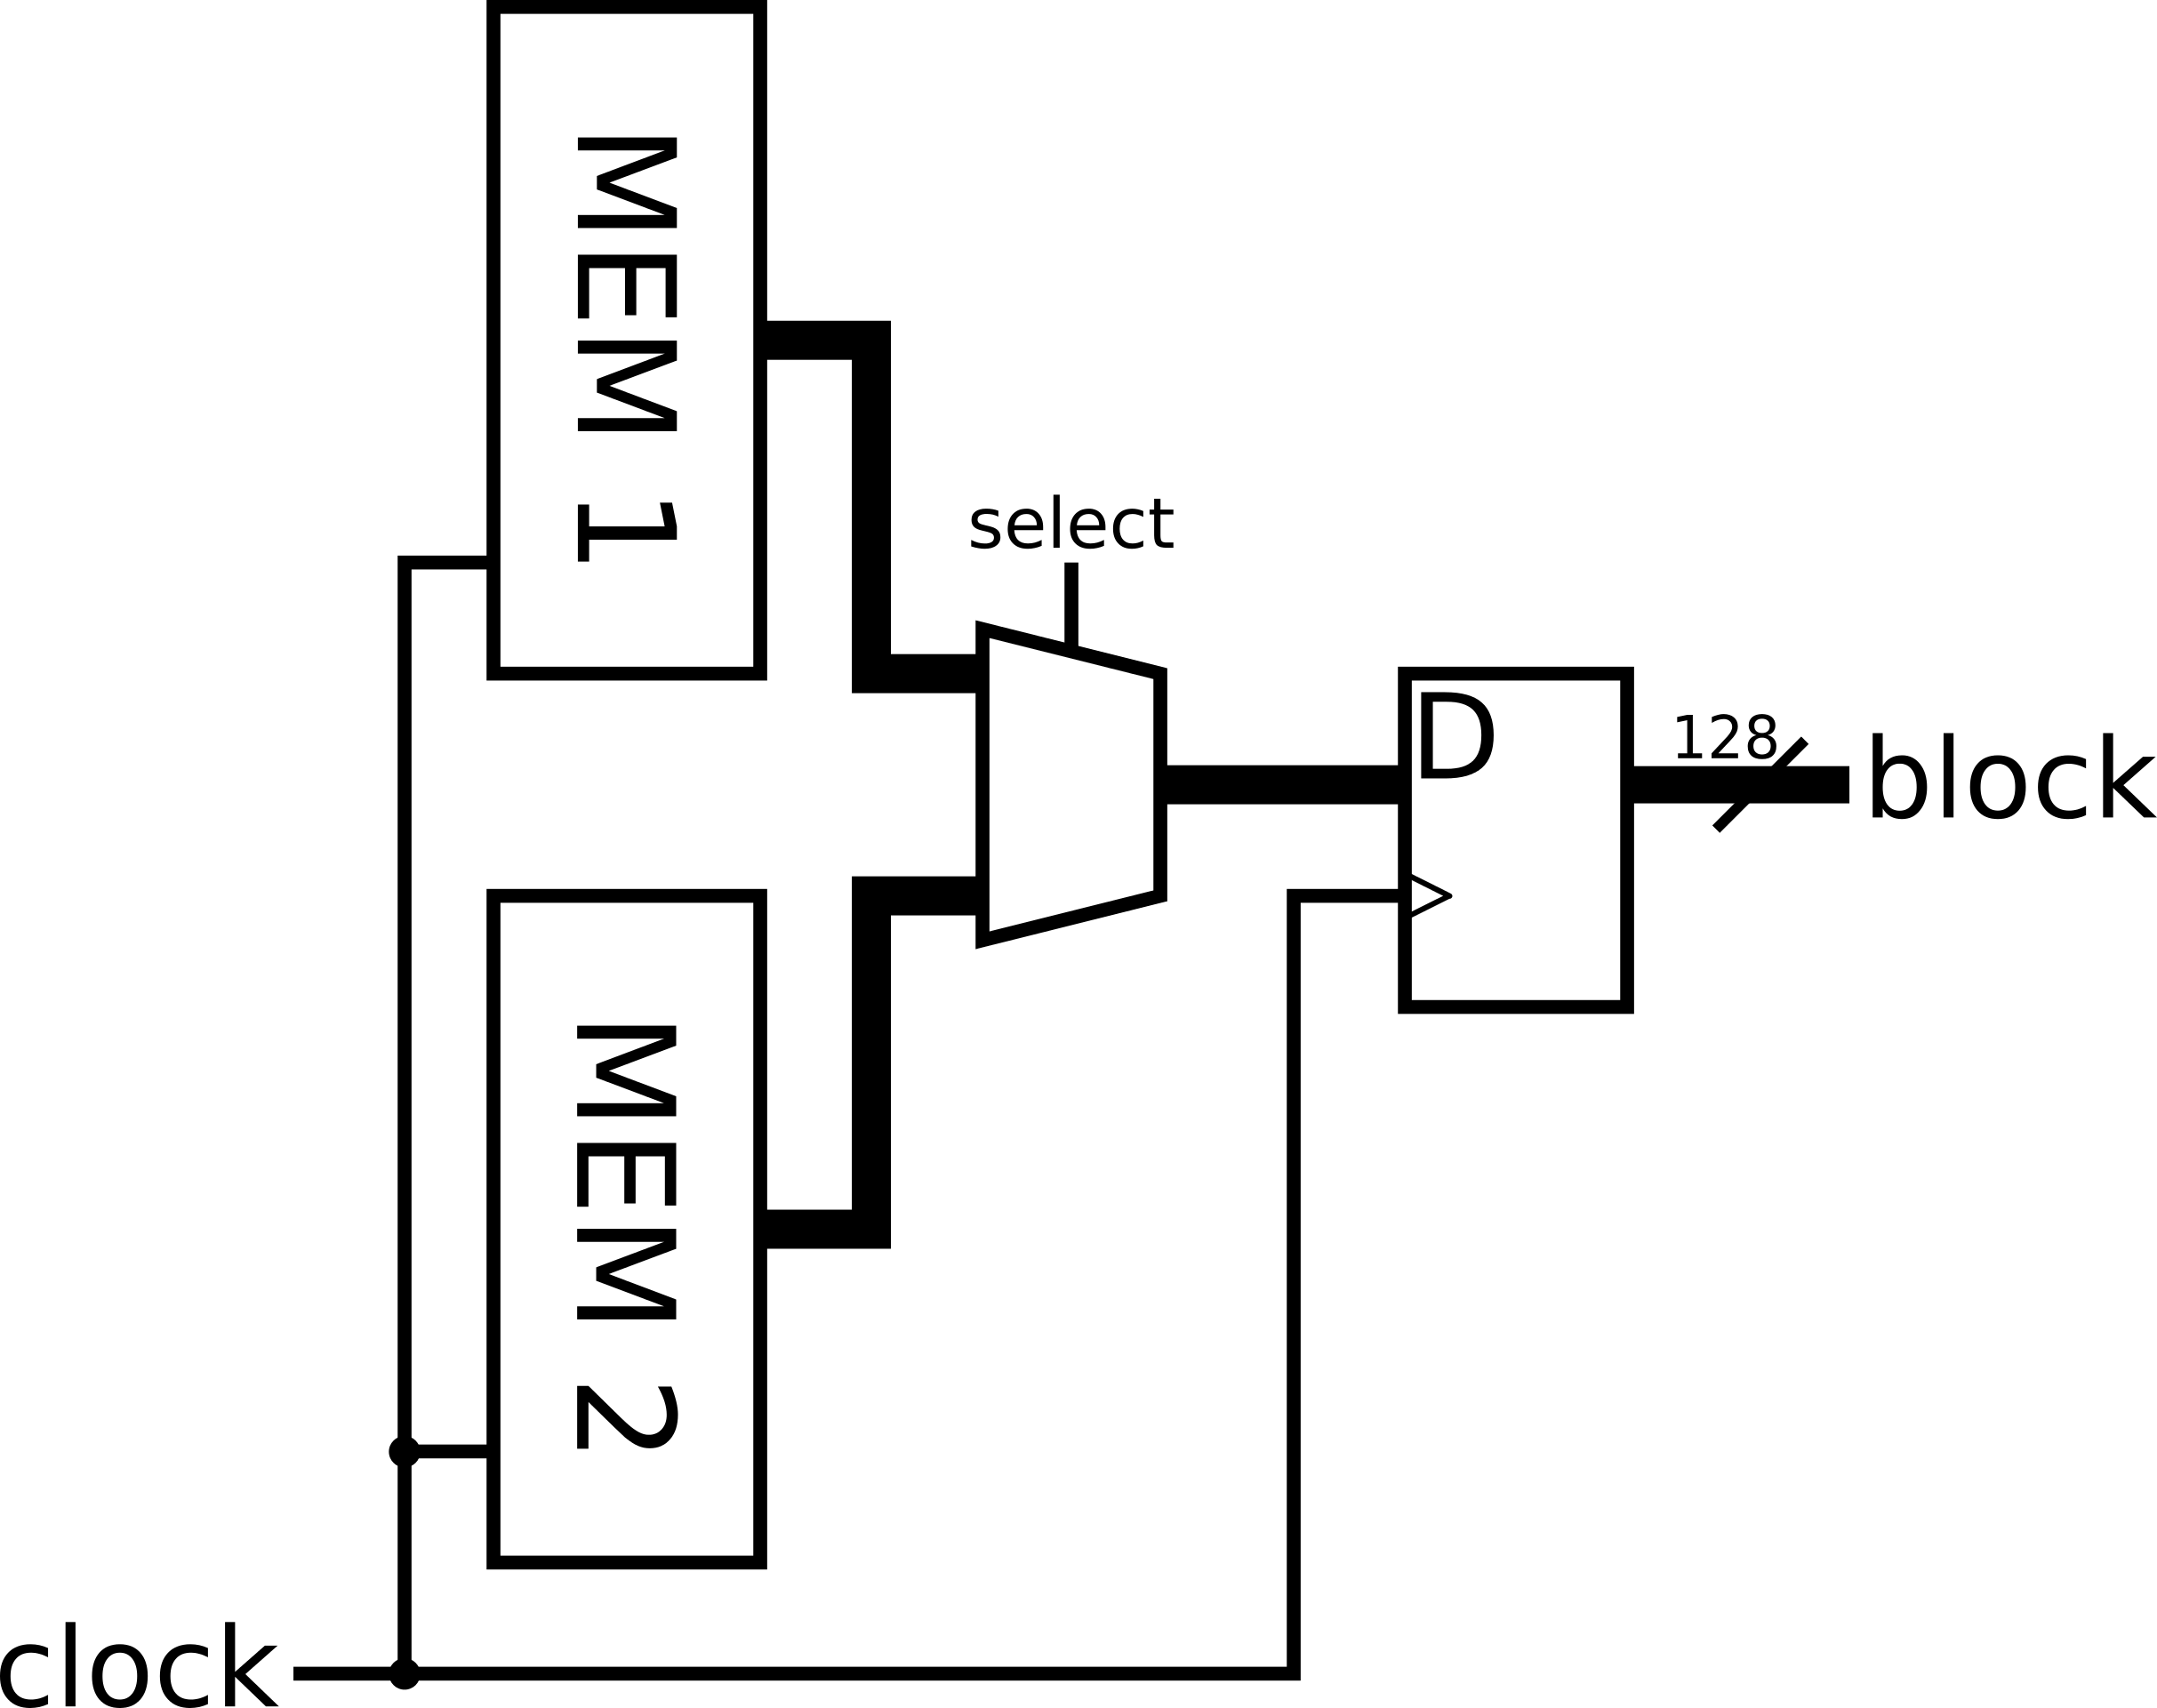
\includegraphics[scale=3]{memory-arrangement}
\caption{Memory solution based on multiplexer}
\label{fig:memory-arrangement}
\end{figure}

Using more banks of ROM was tesed, but adding more resulted in decreased performance due to lack of enough routing resources in FPGA. This testing design was capable of operating at highest frequency and it was chosen to be used for making all frequency measurements.

\subsubsection{Queue based memory solution}
Second testing design (fig. \ref{fig:memory-queue}) that was considered is based on a looped queue of D flip-flops and uses only one bank of ROM - 128 bits wide, 32 blocks deep. Every 33 clock cycles a new block of data is fed to queue at position 0. This results in filling entire queue with test data after $31 * 33 + 1$ clock cycles. After this time stream of testing data is derived from output of one flip-flop in the queue. This approach results in ROM having to operate at only $\frac{1}{33}$ of main clock frequency. This design for delivering data blocks to test module allows for operation at 520MHz. 

\begin{figure}[!h]
\centering
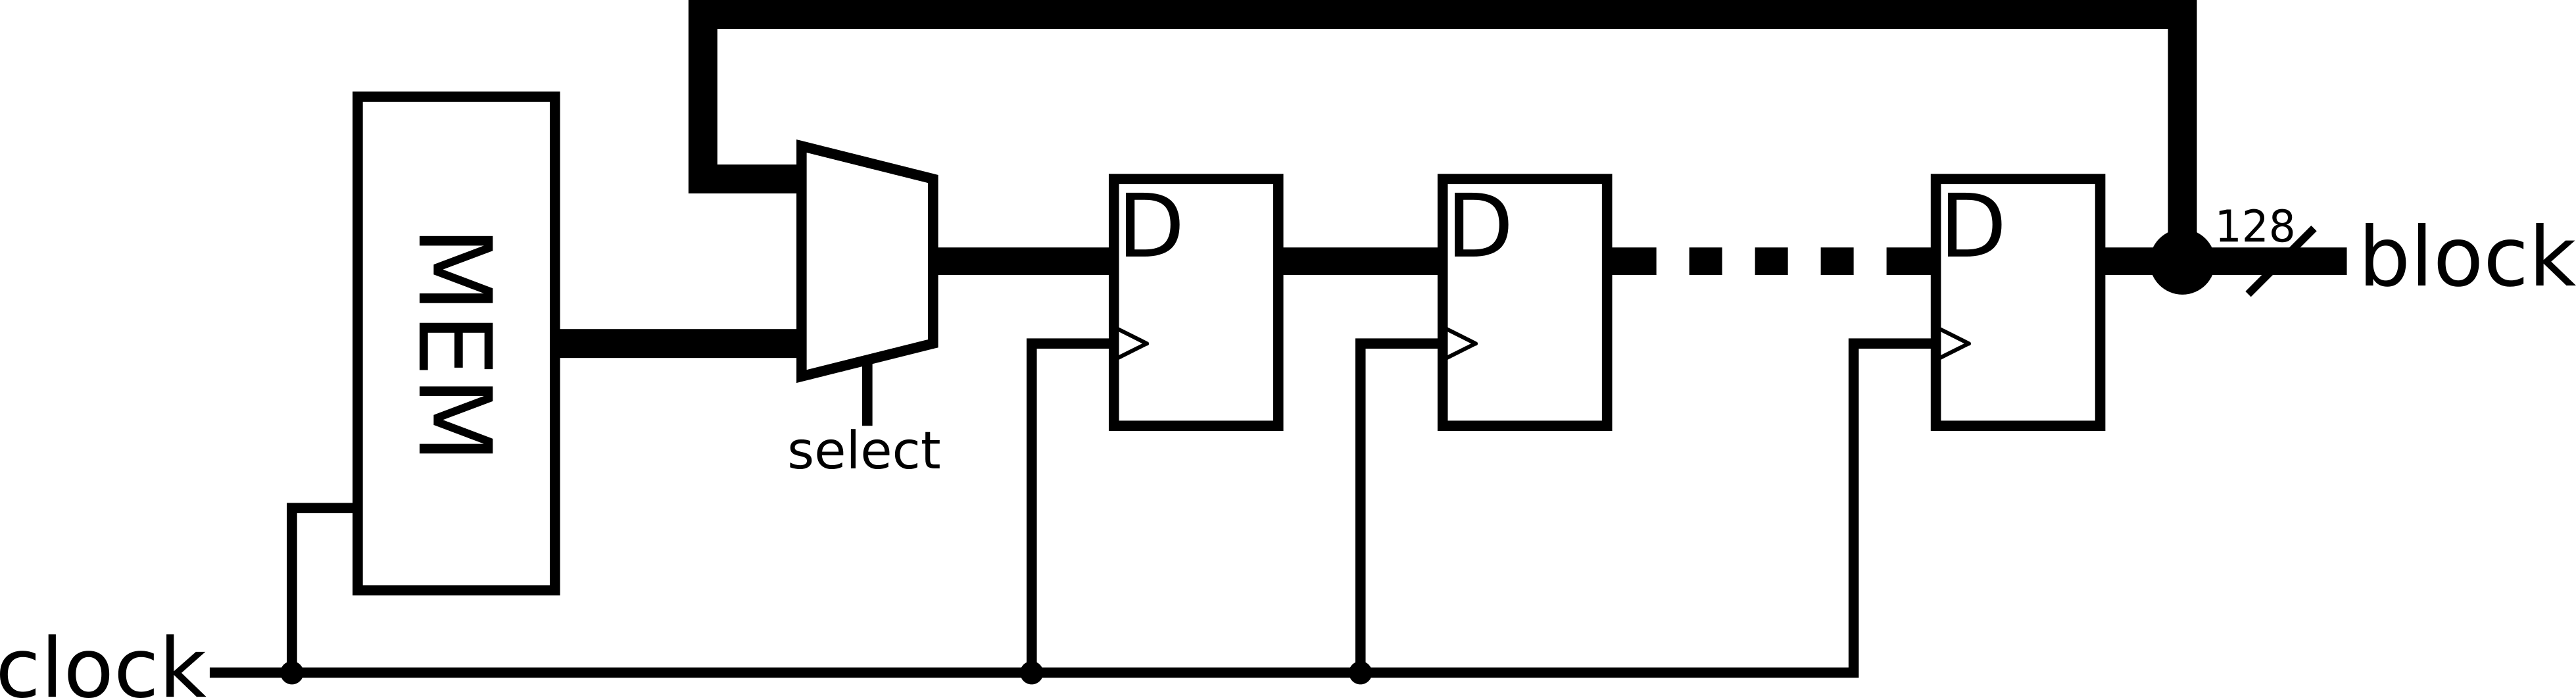
\includegraphics[scale=3]{memory-queue}
\caption{Memory solution based on queue}
\label{fig:memory-queue}
\end{figure}

Other similar designs with varying ROM depths and queue lenghts were tested, but they all performed similarly, and none of them were faster than multiplexer approach.


\subsubsection{Testing circuit}
Testing circuit (fig. \ref{fig:test-circuit}) provides blocks of plaintext and encryption keys to tested design, and compares (using $xor$ gates) calculated cyphertext with expected result. If a bit difference occurs, then tested circuit is considered unstable at given frequency.

\begin{figure}[!h]
\centering
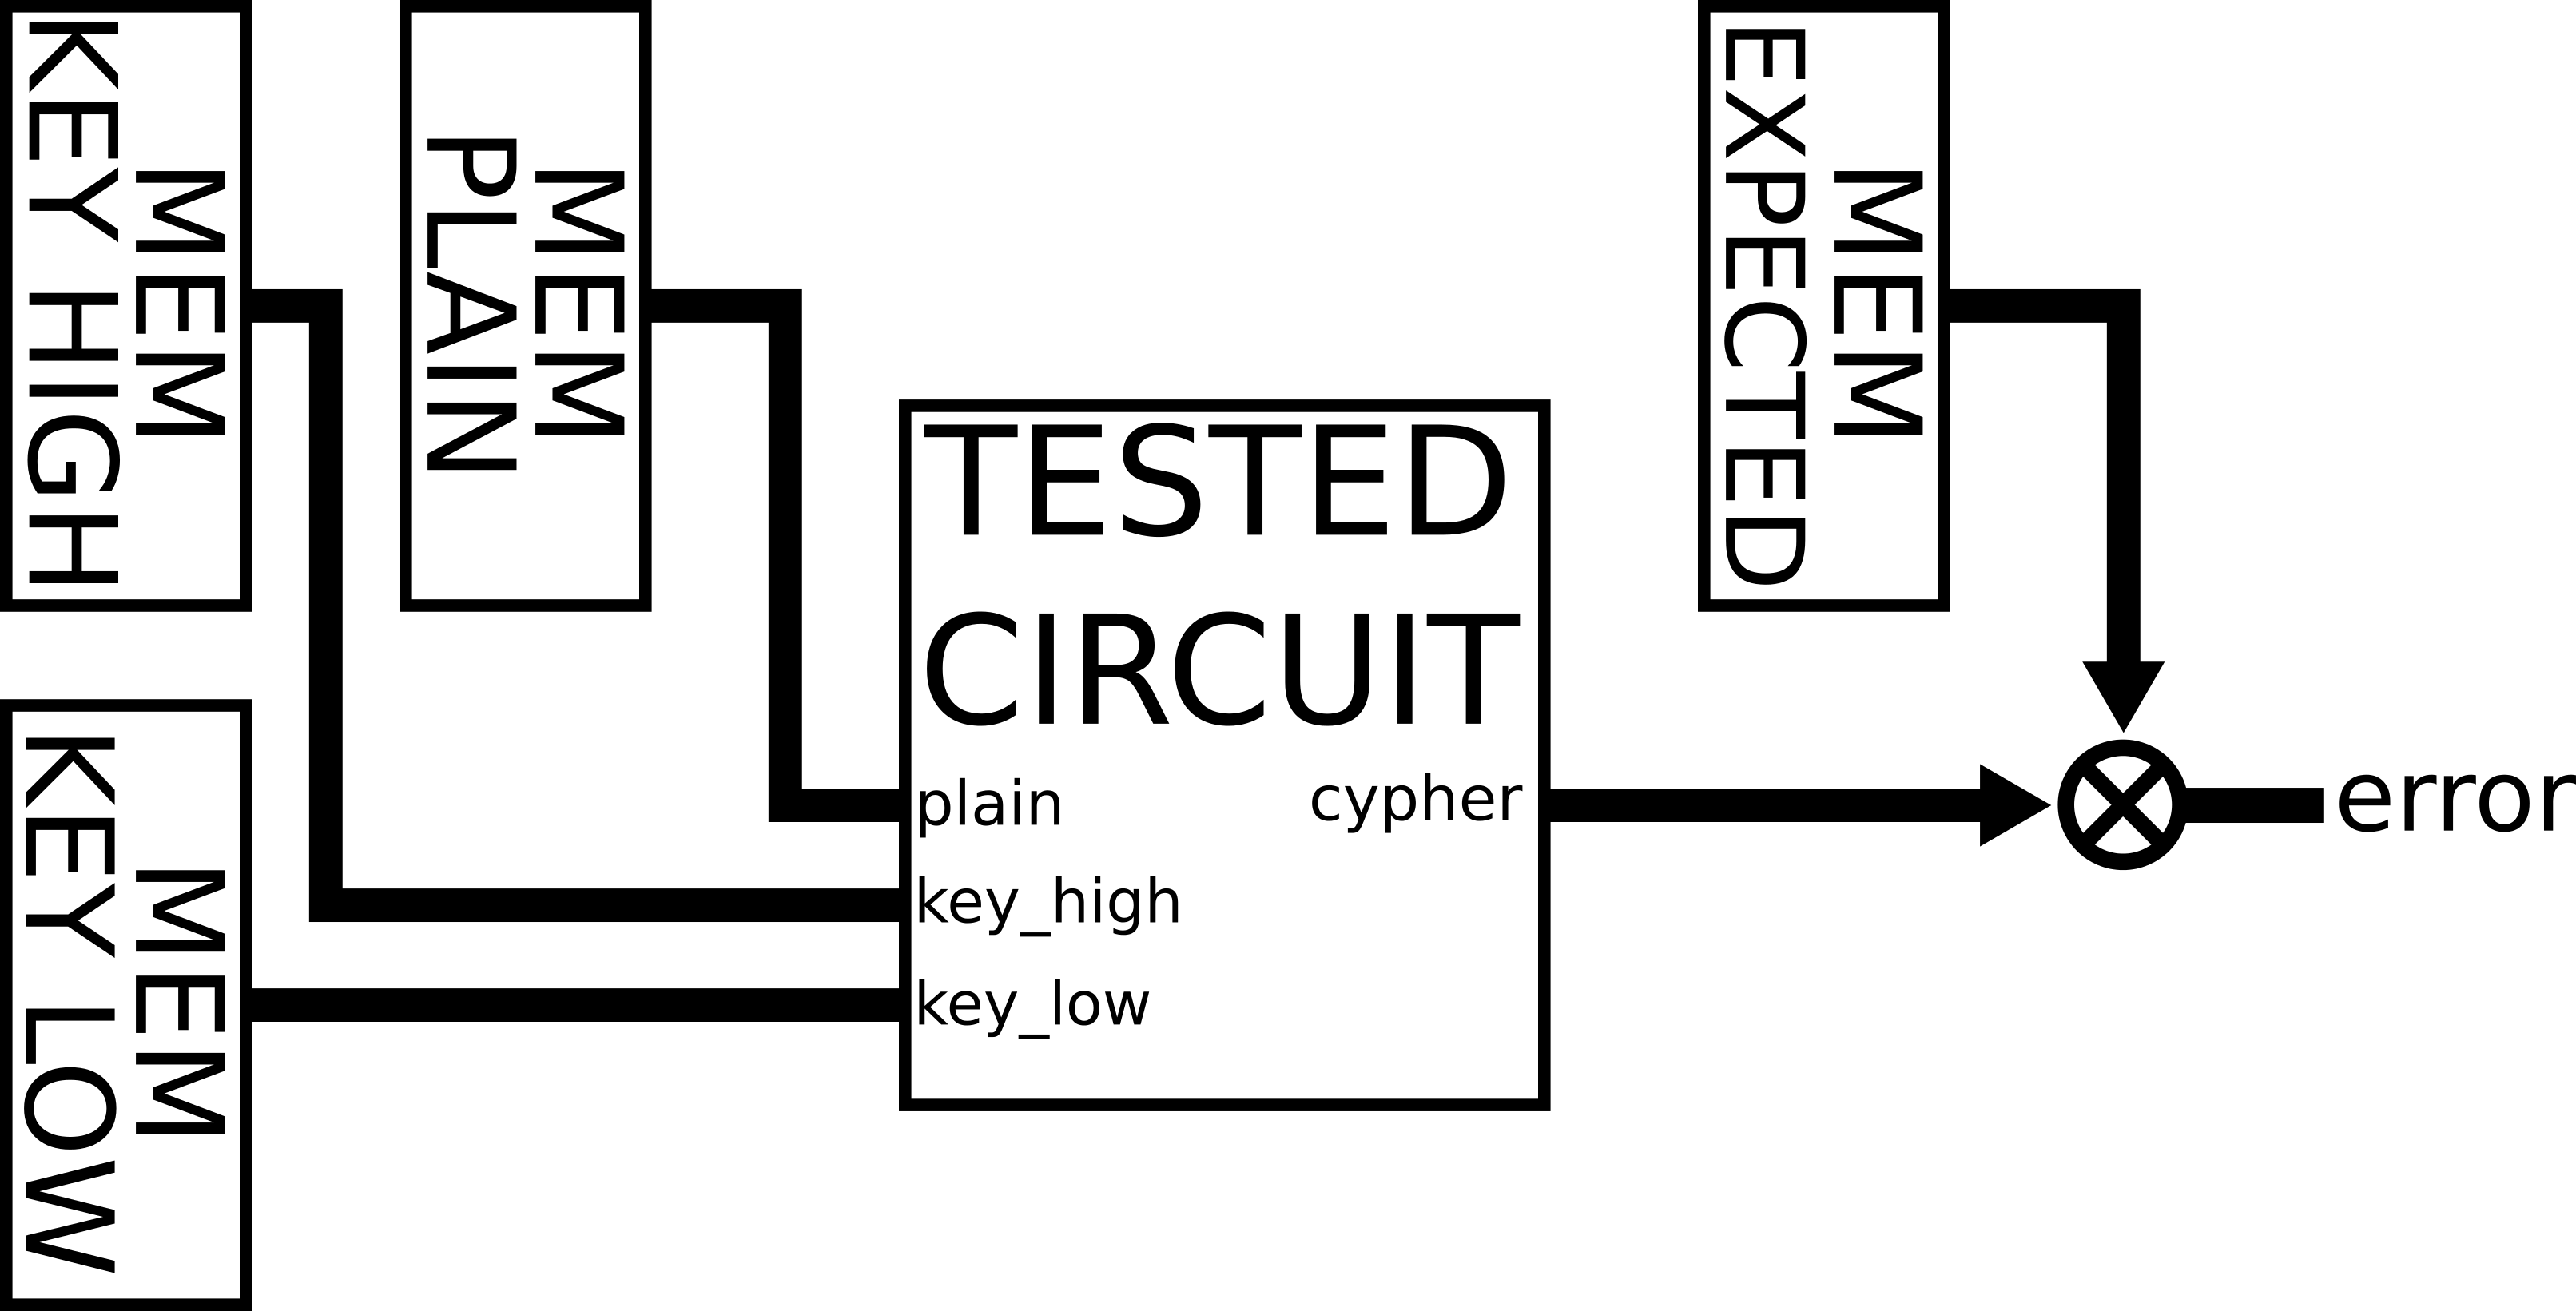
\includegraphics[scale=3]{test-circuit}
\caption{Testing circuit}
\label{fig:test-circuit}
\end{figure}

Data in expected result memory is initiated with an offset taking into account the number of pipeline stages in tested design.

This testing circuits consumes 806 ALM FPGA resources and 32768 on-chip memory bits.



\subsection{Logic utilization}
Logic utilization for each design was calculated based on compiler output - after each compilation Quartus software calculates how many FPGA logic elements the design uses. For each tested design number of logic elements in testing circuit (806) was subtracted to determine how much logic the actual AES encryption module utilizes.



\subsection{Correctness}
Correctness of the design was tested in two ways:
\begin{description}
\item[Wave form simulations] were used for simulating and testing sections of the design. This kind of testing was performed during development process.
\item[Testing of designs deployed in FPGA] was always performed along with performance testing (fig. \ref{fig:test-circuit}). Those tests were performed only after implementation of given part of circuit was completed and wave form simulation testing showed no issues.
\end{description}

Input data and expected results for testing of transformations, key expansion and entire encryption algorithm were taken from examples in AES encryption standard \cite{aes-standard}. For testing of smaller portions of the design input data was randomly generated and expected results were precalculated either maually or by implementing a utility script in python.
